\documentclass[a4paper,12pt]{article}

%%% Работа с русским языком
\usepackage{cmap}					% поиск в PDF
\usepackage{mathtext} 				% русские буквы в фомулах
\usepackage[T2A]{fontenc}			% кодировка
\usepackage[utf8]{inputenc}			% кодировка исходного текста
\usepackage[english,russian]{babel}	% локализация и переносы

%%% Дополнительная работа с математикой
\usepackage{amsmath,amsfonts,amssymb,amsthm,mathtools} % AMS
\usepackage{icomma} % "Умная" запятая: $0,2$ --- число, $0, 2$ --- перечисление

%% Номера формул
%\mathtoolsset{showonlyrefs=true} % Показывать номера только у тех формул, на которые есть \eqref{} в тексте.
%\usepackage{leqno} % Немуреация формул слева

%% Свои команды
\DeclareMathOperator{\sgn}{\mathop{sgn}}
\newcommand*\Laplace{\mathop{}\!\mathbin\bigtriangleup}

%% Перенос знаков в формулах (по Львовскому)
\newcommand*{\hm}[1]{#1\nobreak\discretionary{}
{\hbox{$\mathsurround=0pt #1$}}{}}

%%% Работа с картинками
\usepackage{graphicx}  % Для вставки рисунков
\graphicspath{{pic/}{images2/}}  % папки с картинками
\setlength\fboxsep{2pt} % Отступ рамки \fbox{} от рисунка
\setlength\fboxrule{1pt} % Толщина линий рамки \fbox{}
\usepackage{wrapfig} % Обтекание рисунков текстом




%%% Работа с таблицами
\usepackage{array,tabularx,tabulary,booktabs} % Дополнительная работа с таблицами
\usepackage{longtable}  % Длинные таблицы
\usepackage{multirow} % Слияние строк в таблице

%%% Теоремы
\theoremstyle{plain} % Это стиль по умолчанию, его можно не переопределять.
\newtheorem{theorem}{Теорема}[section]
\newtheorem{proposition}[theorem]{Утверждение}
 
\theoremstyle{definition} % "Определение"
\newtheorem{corollary}{Следствие}[theorem]
\newtheorem{problem}{Задача}[section]
 
\theoremstyle{remark} % "Примечание"
\newtheorem*{nonum}{Решение}

%%% Программирование
\usepackage{etoolbox} % логические операторы

%%% Страница
\usepackage{extsizes} % Возможность сделать 14-й шрифт
\usepackage{geometry} % Простой способ задавать поля
	\geometry{top=8mm}
	\geometry{bottom=12mm}
	\geometry{left=5mm}
	\geometry{right=5mm}
%
%\usepackage{fancyhdr} % Колонтитулы
% 	\pagestyle{fancy}
 	%\renewcommand{\headrulewidth}{0pt}  % Толщина линейки, отчеркивающей верхний колонтитул
% 	\lfoot{Нижний левый}
% 	\rfoot{Нижний правый}
% 	\rhead{Верхний правый}
% 	\chead{Верхний в центре}
% 	\lhead{Верхний левый}
%	\cfoot{Нижний в центре} % По умолчанию здесь номер страницы

\usepackage{setspace} % Интерлиньяж
%\onehalfspacing % Интерлиньяж 1.5
%\doublespacing % Интерлиньяж 2
%\singlespacing % Интерлиньяж 1

\usepackage{lastpage} % Узнать, сколько всего страниц в документе.

\usepackage{soul} % Модификаторы начертания
\usepackage{epigraph}
\usepackage{hyperref}
\usepackage[usenames,dvipsnames,svgnames,table,rgb]{xcolor}
\hypersetup{				% Гиперссылки
    unicode=true,           % русские буквы в раздела PDF
    pdftitle={hw},   % Заголовок
    pdfauthor={Шишкин Максим},      % Автор
    pdfsubject={Эффект Холла в полуповоднике},      % Тема
    pdfcreator={Создатель}, % Создатель
    pdfproducer={Производитель}, % Производитель
    pdfkeywords={hw}, % Ключевые слова
    colorlinks=true,       	% false: ссылки в рамках; true: цветные ссылки
    linkcolor=red,          % внутренние ссылки
    citecolor=black,        % на библиографию
    filecolor=magenta,      % на файлы
    urlcolor=cyan           % на URL
}

\usepackage{csquotes} % Инструменты для ссылок
\usepackage{cite} % Работа с библиографией
%\usepackage[superscript]{cite} % Ссылки в верхних индексах
%\usepackage[nocompress]{cite} % 

\usepackage{float} %force establishe parametr to figure H,h,!

\usepackage{multicol} % Несколько колонок

\usepackage{ mathrsfs }

\usepackage{physics}

\usepackage{mathtools}

\usepackage{empheq}
\usepackage{floatflt}
\usepackage[most]{tcolorbox}
\usepackage{enumerate}

%\usepackage{floatrow}


\usepackage{tikz}
\usetikzlibrary{fadings}
\usetikzlibrary{shadows.blur}
\usetikzlibrary{shapes}

\usepackage{nicematrix}
\NiceMatrixOptions{transparent,nullify-dots}

\usepackage{pgfplots}
\DeclareUnicodeCharacter{2212}{−}
\usepgfplotslibrary{groupplots,dateplot}
\usetikzlibrary{patterns,shapes.arrows}
\pgfplotsset{compat=newest}

\usepackage{pgf}

\author{Максим Шишкин.}
\title{Rectangle viscous flow.}
\date{\today}

\begin{document}

\maketitle
\problem{Найти периодическое движение вязкой несжимаемой жидкости в канале прямоугольной формы.}

Пусть ось, вдоль которой течет жидкость - ось $z$, сечение описывается прямоугольником т.ч. $x\in(0,b)\; y\in (0,s)$.
Получим решение в предположении наличия только $u_z$ компоненты скорости.
Из уравнения несживаемости ($\partial_k u_k=0$), получаем $u_z = u_z(x,y)$.

Тогда уравнение Навье-Стокса для вязкой несжимаемой жидкости принимает простой вид:
\begin{equation}\label{eq:navie-stoks}
    \partial_t \mathbf{u} =- \frac{\nabla p}{\rho} + \nu \Laplace{\mathbf{u}}
\end{equation}
Проецируя это уравнение на оси $x,y$ получаем $p=p(z)$. 

Искать будем гармоническое решение, т.е. $u_z = \real f(x,y) e^{-i\omega t}$.\footnote{$\real$-операция взятия действительной части. Давление также предполагается гармоническим $p\to \real\, p\, e^{-i\omega t}$}

Подставляя такой анзац получаем уравнение на амплитуду:
\begin{equation}
    -i\omega  f = -\frac{\partial_z p}{\rho} + \nu \Laplace{f}\implies \frac{\partial_z p}{\rho} = (i\omega + \nu\Laplace)f
\end{equation}
Проведем явное обезразмеривание полученного уравнения:
 $x = b(\Tilde{x}-\frac{1}{2})$,
 $y = s(\Tilde{y}-\frac{1}{2})$,
 $f = \frac{b^2\partial_z p}{\eta} \Tilde{f}$,
 $\omega = \frac{\nu}{b^2}\Tilde{\omega}$
Далее для удобства тильды не ставятся, кроме того, введем безаразмерное отношение сторон канала $\beta = \frac{b}{s}$.
В безразмерных переменных уравнение переписывается в виде:
\begin{equation}\label{eq:eq_dimen}
    (i\omega + \partial_{x}^2 + \beta^2 \partial_y^2)f=1, \; \eval{f}_{x=\pm\frac{1}{2} \text{ or } y=\pm\frac{1}{2}} = 0 
\end{equation}
    Поскольку симметрия в плоскости нарушена, пробуем найти решение для её 'бесконечного' нарушения \\$\beta=0$.
    В этом случае $f = f_p (x)$. $(\partial_x^2 +i\omega)f_p = 1$. Общее решение дается выражением типа $f_p = \frac{1}{i\omega} + c_+ e^{\lambda x} + c_- e^{-\lambda x}$, где $\lambda = \sqrt{-i\omega} = \sqrt{\omega/2}(1-i)$.
    Для удовлетворения граничным условиям при $x=\pm \frac{1}{2}$ получаем \begin{equation}\boxed{f_p = \frac{1}{i\omega}\left(1-\frac{\cosh{\lambda x}}{\cosh{\frac{\lambda}{2}}}\right)}\end{equation}

Решение же первоночальной задачи можно представить в виде суммы найденного и добавки $f = f_p + f_o$.
Для $f_o $ получаем однородное уравнение \eqref{eq:eq_dimen}, но уже с граничными условиями в виде $\eval{f_o}_{x=\pm \frac{1}{2}}=0$, а $\eval{f_o} _{y=\pm\frac{1}{2}} = -f_p$\footnote{То есть дополнительное решение поправляет ненулевую скорость на второй границе.}
Однородное уравнение допускает разделение переменных $f_n = X(x)Y(y)$, после подстановки и деления на $f_n$ получаем :
\begin{equation}
    i\omega + \underbrace{\frac{\partial_x^2 X}{X}}_{-k_x^2} +\beta^2 \underbrace{\frac{\partial_y^2 Y}{Y}}_{\lambda_y^2}=0
\end{equation}
Как легко видеть $X_n = \sin(k_x (x-\frac{1}{2}))$ причем $k_x = \pi n$, $n\in \mathbb{N}$. \footnote{Разумеется, это представляет стоячую волну в направлении $x$.}
Тогда $\underline{\lambda_y^2 = \beta^{-2}(k_x^2 - i\omega)}$.

Соответственно $Y_n = \dfrac{\cosh{\lambda_y y}}{\cosh{\frac{\lambda_y}{2}}}$

Тогда итоговая $f_o = \sum_n  c_n X_n Y_n$, для удовлетворения второму граничному условию получаем 
\begin{equation}
    \sum_n c_n X_n = - f_p
\end{equation}
Таким образом остался чисто технический момент - получить разложение $f_p$.
В силу того, что $\{X_n\}$ является решением спектральной задачи для эрмитового оператора, они ортогональны относительно скалярного произведения в $L_2(-\frac{1}{2},\frac{1}{2}, \dd{x})$.
Тогда $c_n$ находятся простым проецированием на ортонормированный базис.
\begin{equation}
    c_n = \frac{-2}{i\omega} \int_{-\frac{1}{2}}^{\frac{1}{2}} \left(1-\frac{\cosh{\lambda x}}{\cosh{\frac{\lambda}{2}}}\right) \sin(\pi n \left(x-\frac{1}{2}\right))\dd{x}
\end{equation}
В силу симметрии ясно, что участвует только нечетные $n=2k+1$.
\begin{equation}\boxed{
    c_n = \frac{-4}{i\omega}\left(\frac{\pi n}{-i\omega + (\pi n)^2} - \frac{1}{\pi n}\right) = \frac{-4}{(\pi n)^3 - i\omega (\pi n)}}
\end{equation}
Итого ответ есть 
\begin{equation}\boxed{
    f = \frac{1}{i\omega}
    \left(1-\frac{\cosh{\lambda x}}{\cosh{\frac{\lambda}{2}}}\right) + \sum_{n=2k+1} c_n \sin(\pi n \left(x-\frac{1}{2}\right)) \frac{\cosh{\lambda_y^n y }}{\cosh{\frac{\lambda_y^n}{2}}}} \;,\;  \lambda_y^n = \beta^{-1}\sqrt{(\pi n)^2 - i\omega}, \; \lambda = \sqrt{-i\omega}
\end{equation}
\begin{quote}
    Рассмотрим отдельно стационарный случай, соответствующий $\omega=0$.
    $f_p = \frac{1}{2}(x^2 - \frac{1}{4})$, $c_n = \frac{-4}{(\pi n)^3}$.
    При этом $\lambda_y = \beta^{-1} k_x = \beta^{-1} \pi n$. Если $\beta \to 0$, видно, что $Y_n$ экспоненциально затухает от границы $y=\pm \frac{1}{2}$  с характерным масштабом порядка $\frac{\beta}{\pi n}$, что порядка поперечного масштаба $b$ при возвращении к размерным единицам.
\end{quote}
Не составляет труда сосчитать и поток- среднюю скорость:
\begin{equation}
    Q = \bar{f}=\int_{\fbox{}} \dd{x}\dd{y} f = \frac{1}{i\omega} \left(1-\frac{\tanh{\lambda/2}}{\lambda/2}\right) - \sum_{n=2k+1}c_n\left(\frac{2}{\pi n}\right)\frac{\tanh{\lambda_y^n/2}}{\lambda_y^n/2}
\end{equation}

Теперь предлагается насладиться картинками.
\newpage
\begin{figure}[H]
\begin{center}
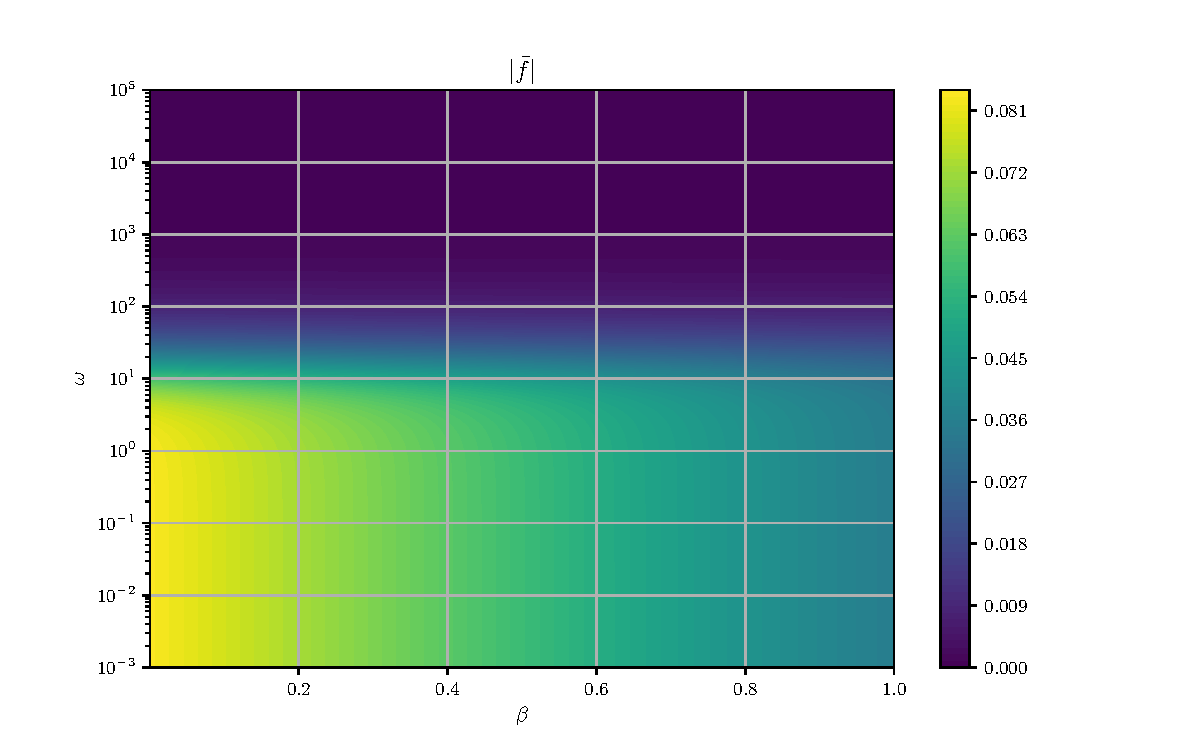
\includegraphics[scale=0.8]{Abs pic conduct.pdf}
\caption{Зависимость модуля средней по сечению безразмерной скорости от параметров(Что-то вроде гидропроводимости). Для стационарного случая $\omega=0$ и плоскости $\beta=0$ эта величина есть $\frac{1}{12}\approx 0.083$} %% подпись к рисунку
\label{ris:experimoriginal} %% метка рисунка для ссылки на него
\end{center}
\end{figure}

\begin{figure}[H]
\begin{center}
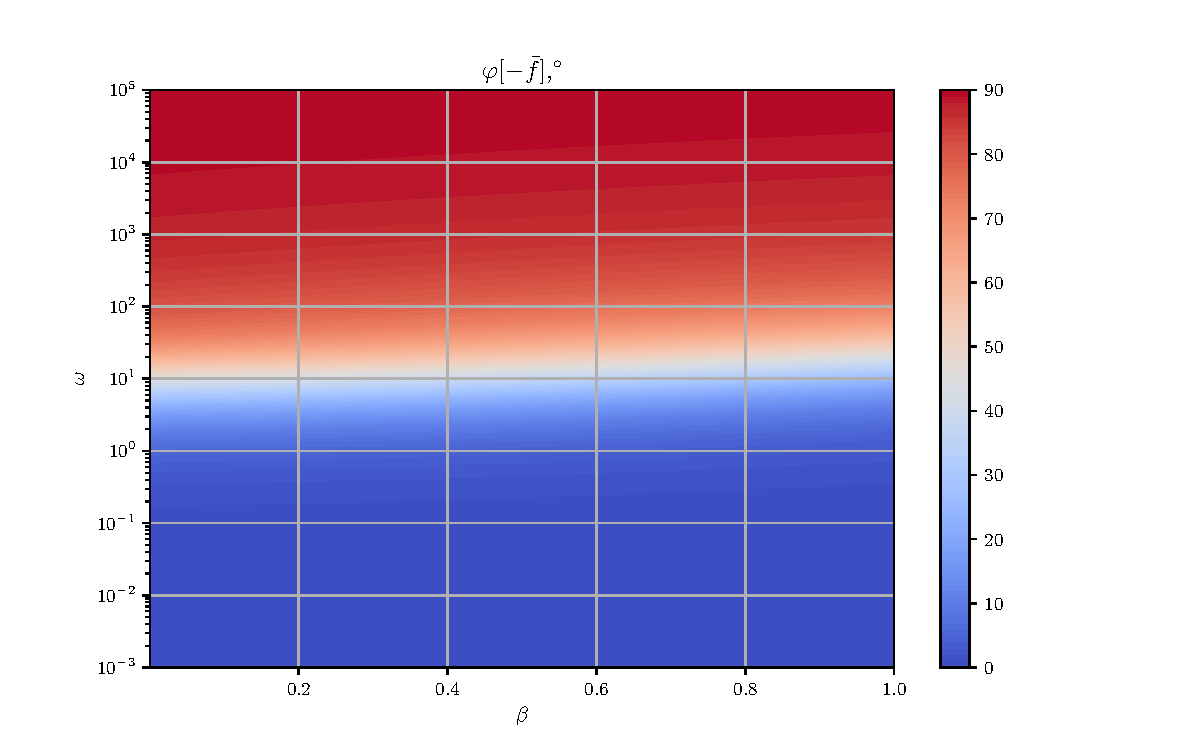
\includegraphics[scale=0.8]{Phase pic conduct.pdf}
\caption{Фаза между средней скоростью и градиентом давления}.
\label{fig:conduct}
\end{center}
\end{figure}

%\begin{figure}[ht!]  
%\vspace{-4ex} \centering \subfigure[]{
%\includegraphics[width=0.45\linewidth]{Abs %W=0.01_Beta=1.pdf} \label{fig:Abs W=0.01_Beta=1} }  
%\hspace{4ex}
%\subfigure[]{
%\includegraphics[width=0.45\linewidth]{Phase %W=0.01_Beta=1.pdf} \label{fig:Phase W=0.01_Beta=1} }
%\caption{Модуль скорости \subref{fig:Abs W=0.01_Beta=1} и %фаза в градусах \subref{fig:Phase W=0.01_Beta=1} %относительно центра - случай квадрата($\beta=1$).} %\label{fig:W=0.01_Beta=1}
%\end{figure}
\newpage 

\begin{figure}[H]
\begin{minipage}[h]{0.47\linewidth}
\center{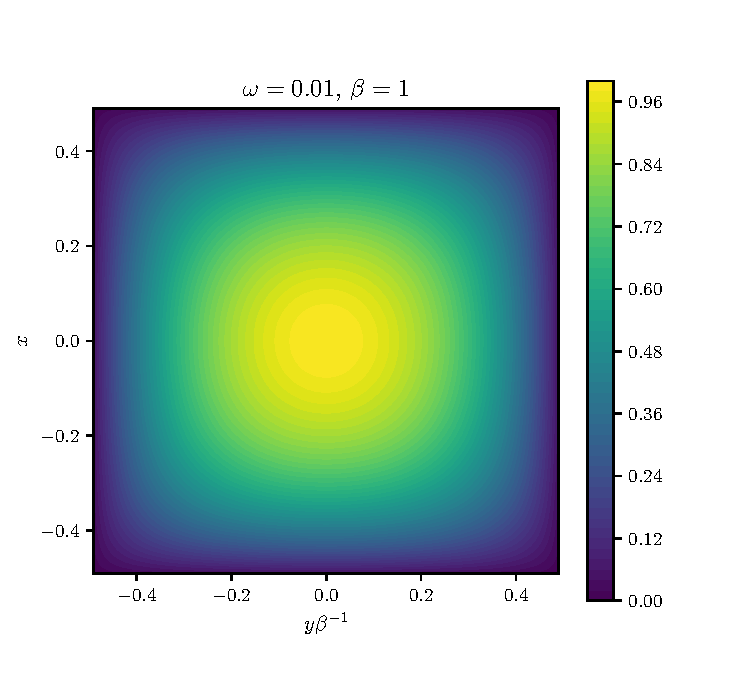
\includegraphics[width=1\linewidth]{Abs W=0.01_Beta=1.pdf}}   \small a)\\
\end{minipage}
\hfill
\begin{minipage}[h]{0.47\linewidth}
\center{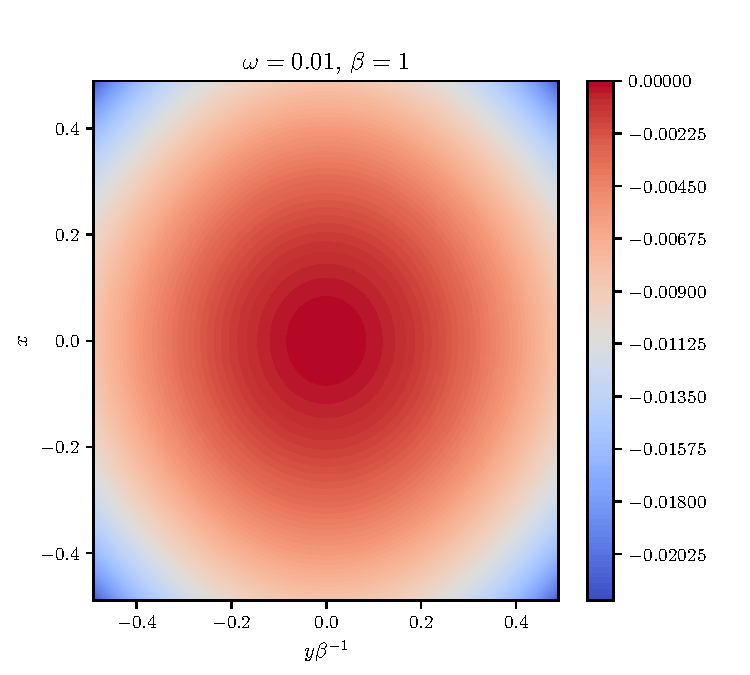
\includegraphics[width=1\linewidth]{Phase W=0.01_Beta=1.pdf}}  \small d)\\
\end{minipage}
\vfill
\begin{minipage}[h]{0.47\linewidth}
\center{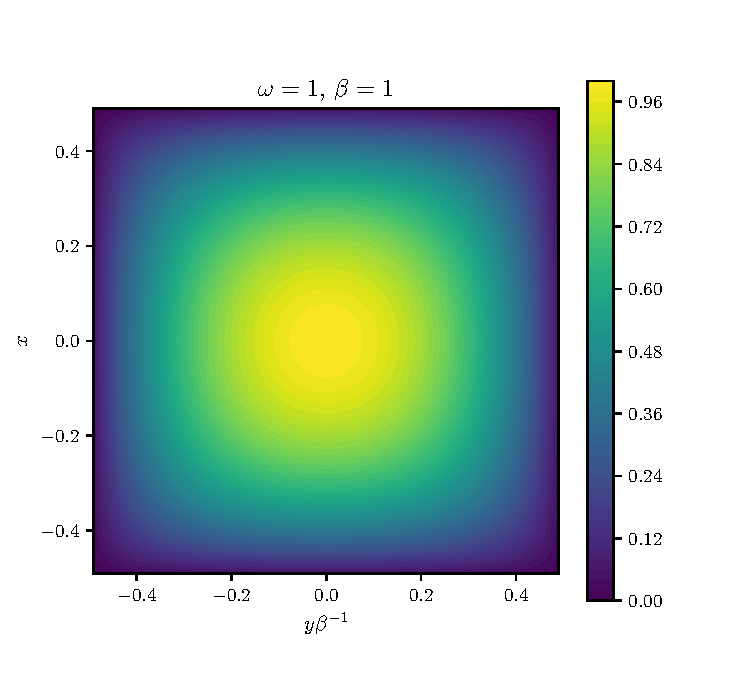
\includegraphics[width=1\linewidth]{Abs W=1_Beta=1.pdf}} \small b) \\
\end{minipage}
\hfill
\begin{minipage}[h]{0.47\linewidth}
\center{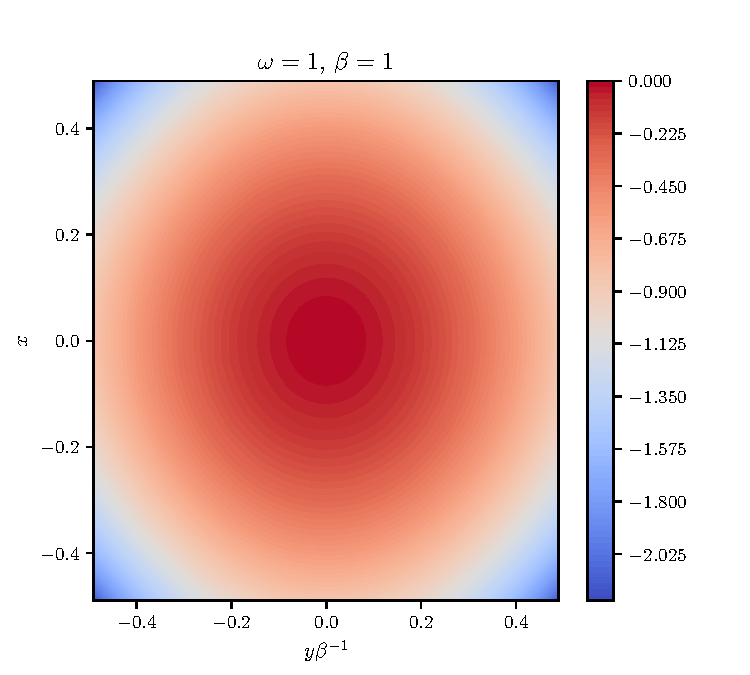
\includegraphics[width=1\linewidth]{Phase W=1_Beta=1.pdf}} \small e) \\
\end{minipage}
\vfill
\begin{minipage}[h]{0.47\linewidth}
\center{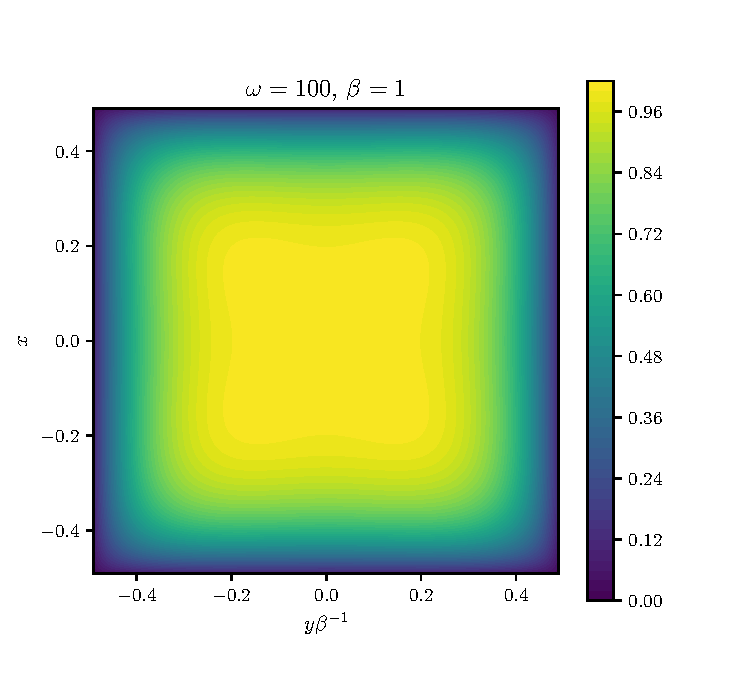
\includegraphics[width=1\linewidth]{Abs W=100_Beta=1.pdf}} \small c) \\
\end{minipage}
\hfill
\begin{minipage}[h]{0.47\linewidth}
\center{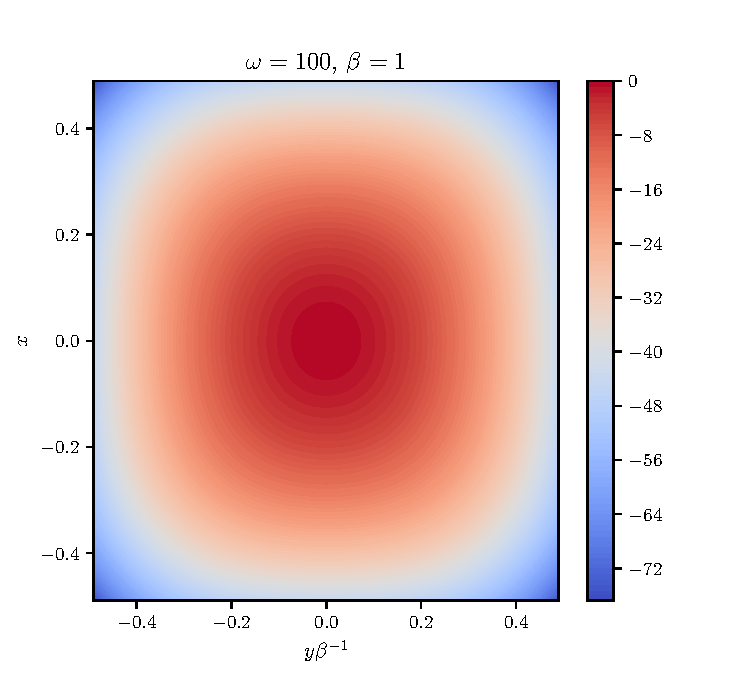
\includegraphics[width=1\linewidth]{Phase W=100_Beta=1.pdf}} \small f) \\
\end{minipage}
\caption{Поля скоростей (a-c) и фазы в градусах (d-f) для квадратного канала.}
\end{figure}


\begin{figure}[H]
\begin{minipage}[h]{\linewidth}
\center{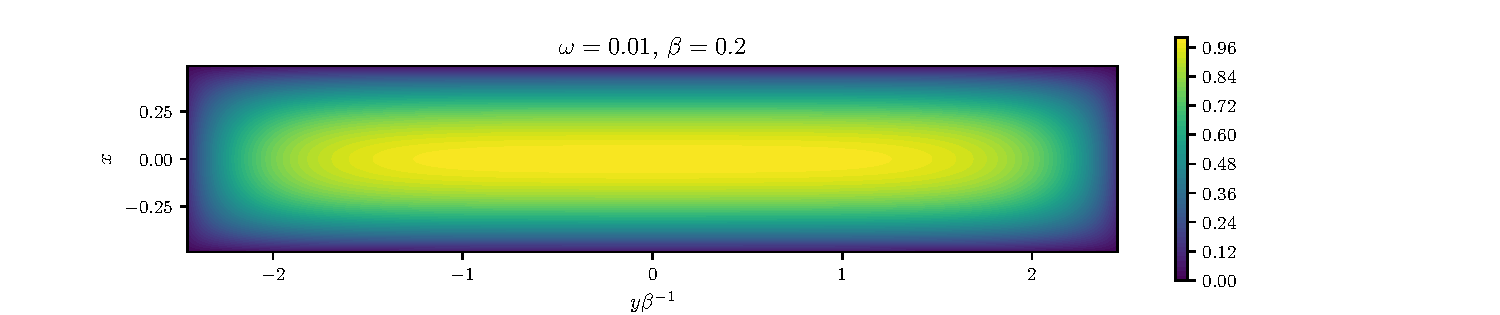
\includegraphics[width=0.8\linewidth]{Abs W=0.01_Beta=0.2.pdf}}   \center{ \small a)}\\
\end{minipage}
\vfill
\begin{minipage}[h]{\linewidth}
\center{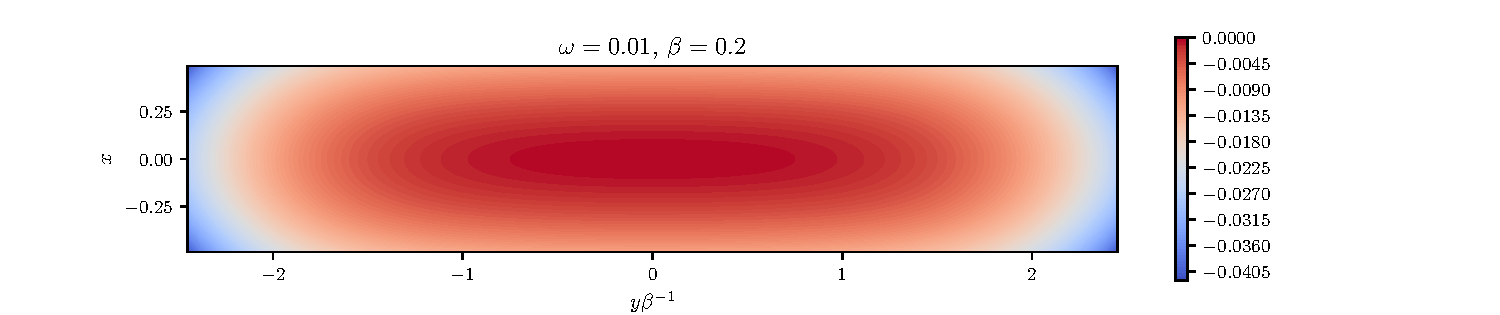
\includegraphics[width=0.8\linewidth]{Phase W=0.01_Beta=0.2.pdf}}  \center{ \small d)}\\
\end{minipage}
\vfill
\begin{minipage}[h]{\linewidth}
\center{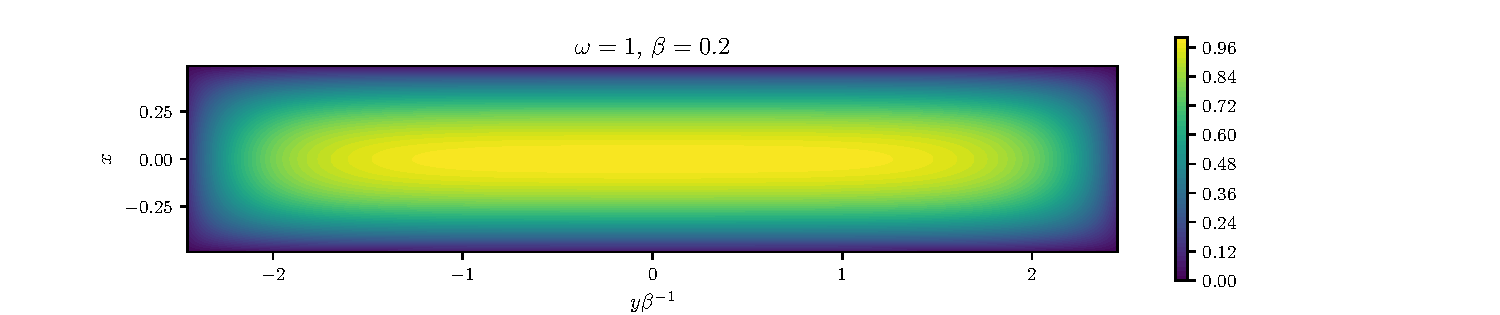
\includegraphics[width=0.8\linewidth]{Abs W=1_Beta=0.2.pdf}} \center{\small b)} \\
\end{minipage}
\vfill
\begin{minipage}[h]{\linewidth}
\center{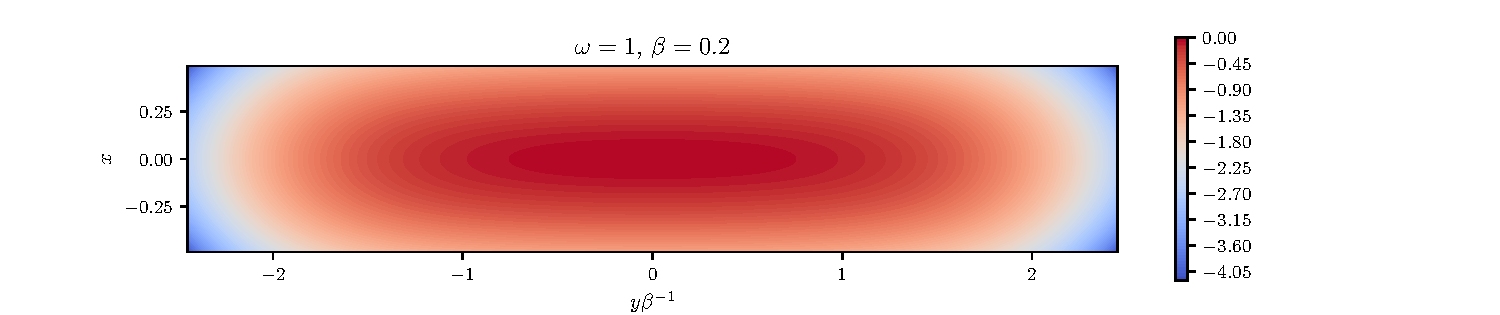
\includegraphics[width=0.8\linewidth]{Phase W=1_Beta=0.2.pdf}} \center{\small e)} \\
\end{minipage}
\vfill
\begin{minipage}[h]{\linewidth}
\center{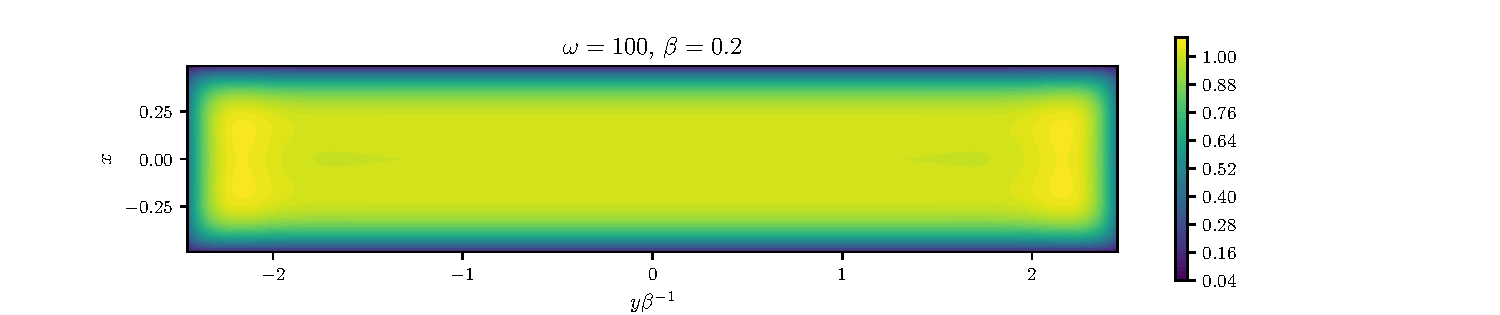
\includegraphics[width=0.8\linewidth]{Abs W=100_Beta=0.2.pdf}} \center{\small c)} \\
\end{minipage}
\vfill
\begin{minipage}[h]{\linewidth}
\center{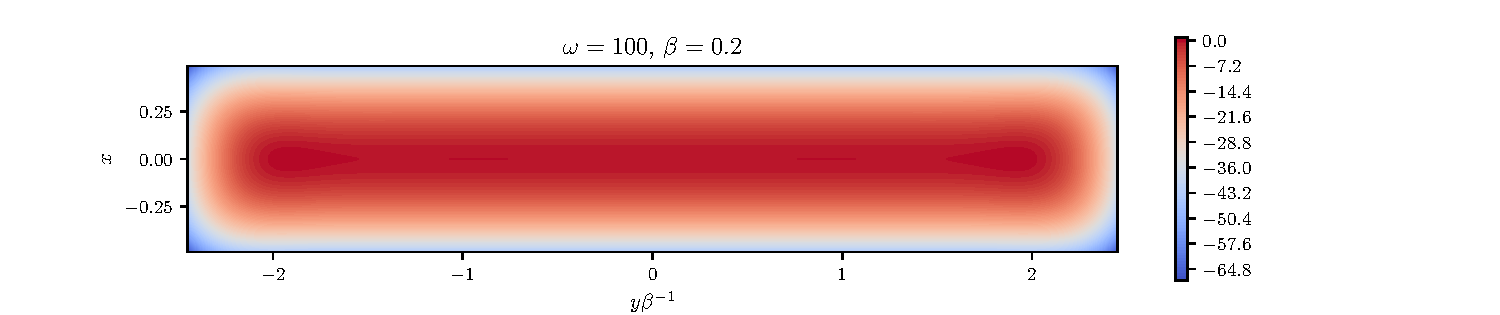
\includegraphics[width=0.8\linewidth]{Phase W=100_Beta=0.2.pdf}} \center{\small f)} \\
\end{minipage}
\caption{Поля скоростей (a-c) и фазы в градусах (d-f) для прямоугольного канала.}
\end{figure}
\newpage
Перейдём к более подробному исследованию случая бесконечного по оси $y$ канал ($\beta=0$).
\begin{figure}[H]
    \centering
    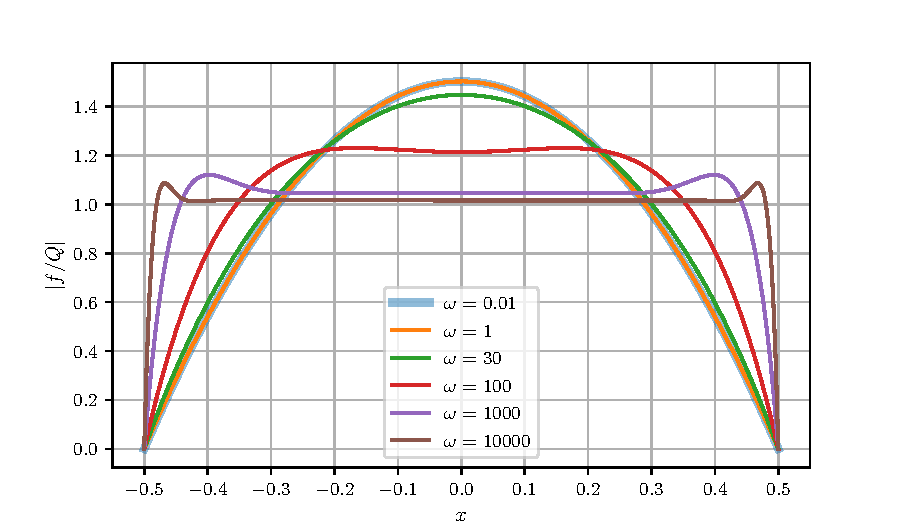
\includegraphics[]{Abs plane.pdf}
    \caption{Распределение модуля скорости(отнормированно на среднюю) в случае плоского канала}
    \label{fig:abs plane}
\end{figure}
\begin{figure}[H]
    \centering
    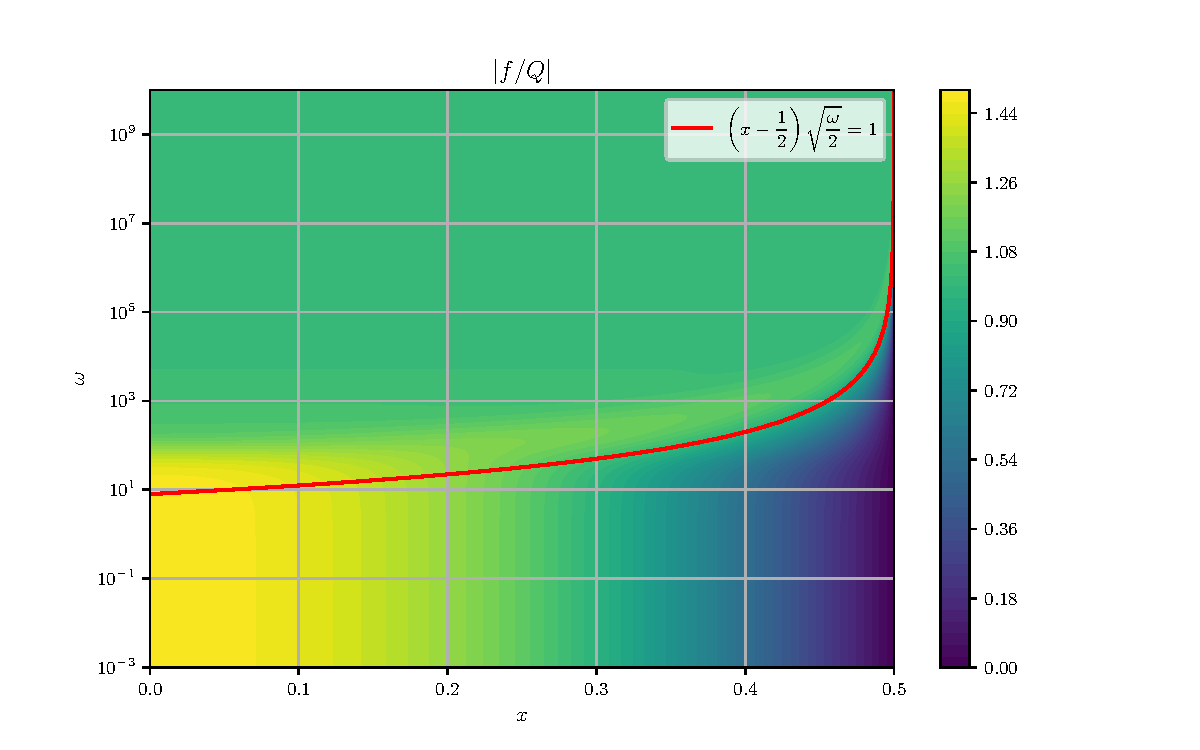
\includegraphics[]{Abs pic plane.pdf}
    \caption{Распределение модуля скорости(отнормированно на среднюю) в случае плоского канала в зависимости от частоты. Кривой показана огибающая области неоднородного течения для высокочастотной области.}
    \label{fig:abs plane pic}
\end{figure}

\begin{figure}[H]
    \centering
    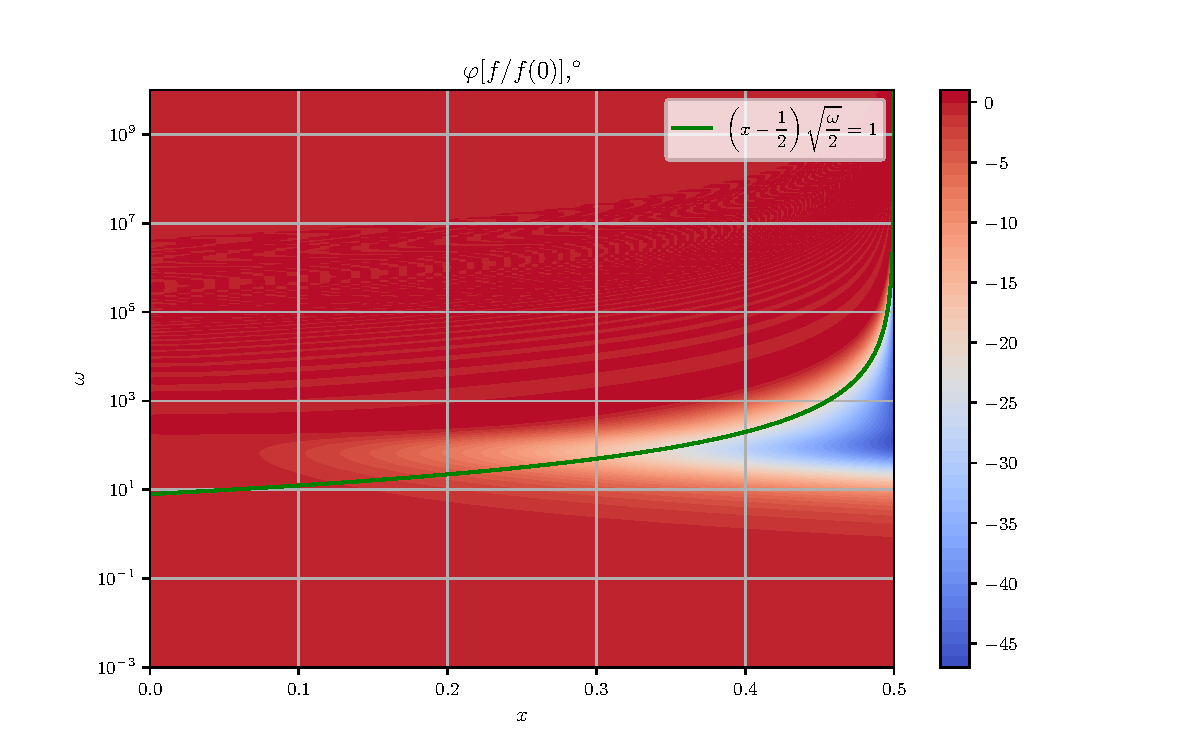
\includegraphics[]{Phase pic plane.pdf}
    \caption{Распределение фазы скорости(отнормированно фазу в центре) в случае плоского канала в зависимости от частоты. Кривой показана огибающая области неоднородного течения для высокочастотной области.}
    \label{fig:abs plane pic}
\end{figure}
\begin{flushright}
\Large \textbf{Dixi}
\end{flushright}
\end{document}